%% RSAA THESIS 'TEMPLATE' BY JOSHUA RICH <joshua.rich@gmail.com>
%% README:
% This template is designed to be used with pdflatex rather than plain
% latex.  It was developed under a TeXLive 2007 TeX distribution on
% Linux.  

% for requirements of typesetting and formatting see:
% http://info.anu.edu.au/Policies/_REG/Guidelines/PhD_Exam_Theses.asp
% (in emacs, type M-x browse-url with the cursor on 
% the link above)

%%NOTES ABOUT THE DOCUMENT CLASS
% Yes, I'm using a report style.  Any 'thesis style' you might
% find or someone will give you is based on the standard report
% class, but is probably well outdated compared to whatever TeX
% you have installed.  Besides, why use that style file if you 
% have no idea what it actually does?  You will probably just redefine
% all of its customisations anyway...
\documentclass[11pt,twoside,openright, pdftex]{report} 

% define some constants that can be used in various places to easily
% specify title, subjects, author etc.
\newcommand{\thesistitle}{Type Ia Supernovae: Explosions and Progenitors}
\newcommand{\fullname}{Wolfgang Eitel Kerzendorf}
\newcommand{\shortname}{W. E. Kerzendorf}
\newcommand{\thesissubjects}{stars: supernovae: progenitors --- stars: binaries: symbiotic ---
stars: supernovae: individual (SN 1572, SN 1006)}

%%NOTES ABOUT BABEL PACKAGE:
% It requires two components; the 
% \usepackage line above and the language put in the \documentclass.
% 'british' is used because that is the english style required for an
% ANU thesis.  This will ensure LaTeX uses british hyphenation and
% other language constructs when generating the text.  Putting the
% babel usepackage at the very top also ensures other packages called
% through \usepackage can take advantage of babel if they are set up
% for such.  
% We can also do tricky things in our ~/.emacs file if we
% are an emacs user now as well.  Grab the flyspell-babel and
% ispell-multi  emacs packages from:
% http://www.dur.ac.uk/p.j.heslin/Software/Emacs/
% And put it somewhere Emacs can find it (probably under ~/.emacs.d).
% Then add the following lines to your .emacs:
%   (dolist (hook '(LaTeX-mode-hook))
%   (add-hook hook (lambda () (flyspell-mode 1))))
%   (add-hook 'tex-mode-hook (function (lambda () (setq ispell-parser 'tex))))
%   (autoload 'flyspell-babel-setup "flyspell-babel")
%   (add-hook 'latex-mode-hook 'flyspell-babel-setup)
% After this, you should have Emacs auto-suggesting word corrections
% AND doing it in british-english automagically.  You can do a similar trick
% for papers by simply changing 'british' above to 'american', and
% flyspell will check your paper in american-english.
\usepackage[british]{babel}

%\usepackage{hyperref}

% ---------------------------------------------------------------------
% page size and margins
% ---------------------------------------------------------------------
%%NOTES ABOUT GEOMETRY PACKAGE:
% Below is using the geometry package as it is just cool.  This allows
% you to directly specify the margin requirements as outlined by ANU
% directly.  Here the inner border is 4cm and the outer is 2cm.  Top
% and bottom are also 2cm.  This is much easier than trying to work
% out page and margin dimensions by hand.  This is how you should use
% LaTeX...
\usepackage{geometry}
\geometry{a4paper,twoside}
\geometry{includehead,includefoot}
\geometry{hmargin={4cm,2cm}}
\geometry{vmargin={2cm,2cm}}

% ---------------------------------------------------------------------
% miscellaneous packages used
% ---------------------------------------------------------------------
\usepackage[hiresbb]{graphicx}
\DeclareGraphicsExtensions{.pdf}
%\DeclareGraphicsExtensions{.eps}
\usepackage[twoside]{rotating}

%%NOTES ABOUT FONTS PACKAGES:
% The basic requirements for fonts in an ANU thesis demand clear
% readability and that is about all.  So if you choose a nice,
% standard serif font you won't have any problems.
% I several font families in my thesis below:
%  pxfonts: math typesetting
%  tgpagella: for the normal text font (serif)
%  tgheros: for the sans serif font
%  tgcursor: for the typewriter style font
% TeX Gyre Pagella, Heros and Cursor are part of the TeX Gyre family
% of fonts, which can be obtained from:
%   http://www.gust.org.pl/projects/e-foundry/tex-gyre/
% Not all of the TeX Gyre, and possibly not the latest glyphs are
% available in standard TeX distributions.  
%
% The 'mathpazo' package provides an almost identical, albeit not
% actively developed font family to TeX Gyre Pagella and is included
% in standard TeX distributions.  This package
% also provides a full range of math glyphs.  You'd need to find
% alternative sans serif and typewriter fonts to use with this package.
%
% You can see a whole heap of LaTeX fonts, most of which are also in a
% standard TeX distribution at: 
%  http://www.tug.dk/FontCatalogue/
% This web-page shows what each font looks like and what you need to
% do to include the font in your document.  Note it lists fonts that
% may not be installed by your default TeX installation...
%
% Another list of fonts, recommended by `typophiles' can be found at:
%  http://typophile.com/node/18207
% Although the above list includes some really nice fonts, their
% availability in TeX distributions varies.  You may have to install
% them manually...
\usepackage{xfrac}
\usepackage[T1]{fontenc}
\usepackage{textcomp}
\usepackage{ucs}
\usepackage[utf8x]{inputenc}
\usepackage{amsmath,amssymb}
\usepackage{pxfonts}
\usepackage{tgheros,tgpagella}
\renewcommand*\ttdefault{qcr}
\linespread{1.05} % tgpagella/mathpazo need a bigger line spacing
\usepackage{microtype}
% bibliography uses natbib, this will be a requirement
\usepackage[round]{natbib}
% Super-nice looking tables, better than deluxetable
\usepackage{ctable, longtable}
%%NOTES ABOUT CAPTION AND SUBFIG PACKAGES
% I'm using the caption package to style my captions.
% You need to read the documentation for this package (on CTAN) as it
% has simple explanations of the options and examples of what it looks
% like.
%
% The subfig package allows the ability to control in detail
% positioning of sub-plots in a complex figure as well as add labels
% to them, which can then be referenced in the text without the need
% for changing the actual number as your sub-figures change.
% The subfig package inherits options from the caption package, so
% declare them together.
%
\usepackage[l2tabu, orthodox]{nag}
\usepackage[]{caption,subfig}
\usepackage{captcont}
\captionsetup{format=hang,%
%  indention=-1.5cm,%
  labelsep=quad,%
  labelfont={footnotesize,bf},%
  textfont={footnotesize}}
% The hyperref package is a must while editing.  It provides urls
% inside your document; you can then click to go to certain pages,
% figures or bibliography entries.
\usepackage[pdftex,hyperindex, unicode,pageanchor,plainpages=false]{hyperref}
% \hypersetup{pdftitle=\thesistitle\ - \shortname,%
%   pdfauthor=\fullname,%
%   pdfsubject={\thesissubjects},%
%   citecolor=DodgerBlue3,%
%   linkcolor=Ivory4,%
%   anchorcolor=CadetBlue4}
%for printing, make all colours black...
\hypersetup{pdftitle=\thesistitle\ - \shortname,%
pdfauthor={\fullname},%
pdfsubject={\thesissubjects},%
colorlinks=false,%
breaklinks=true,%
bookmarks=true,%
bookmarksnumbered=false,%
%hidelinks
%citecolor=green,%
%filecolor=blue,%
%linkcolor=blue,%
%urlcolor=blue%
}
\usepackage{bookmark}
\usepackage{varioref}
% Drop capitals at the start of chapters
% Allow defining of colours. Useful for:
% - defining the colours of links, citations etc.
% together with hyperref (i.e. in hyperrefsetup)
% - get alternating row colours or shades in tables
\usepackage[hyperref,x11names, table]{xcolor}
\usepackage{xstring}


% Stops figures and tables 'floating' past the section in which they
% are declared.
\usepackage[section]{placeins}
\usepackage[toc,titletoc]{appendix}

%%NOTES ABOUT NAG
% this is a very good package to use.  If you want to write good LaTeX
% code and want to make sure you aren't using outdated methods (like
% your supervisor does), then use this package.  It will complain when
% you use outdated or wrong LaTeX commands.

\usepackage{ifthen}
\usepackage{pseudocode}
\usepackage{chronology}


\usepackage[xindy, toc, hyperfirst=false, sanitize={name=false,description=false,symbol=false}]{glossaries}
%\makeglossaries
\glossarystyle{index}
% ---------------------------------------------------------------------
% command re-definitions and additions
% ---------------------------------------------------------------------

% i.e. -- e.g. -- etc. -- et. al.
\newcommand{\eg}{{\em e.g.,}}
\newcommand{\ie}{{\em i.e.,}}
\newcommand{\etc}{{\em etc.}}
\newcommand{\etal}{{\em et al.}}

% symbols
\newcommand{\HI}{\hbox{\rmfamily H\,{\textsc i}}}
\newcommand{\HIfat}{\hbox{\rmfamily\bfseries H\,{\textsc i}}}
\newcommand{\HIsub}{\hbox{{\scriptsize H}\,{\tiny I}}}
\newcommand{\HII}{\hbox{\rmfamily H\,{\scshape ii}}}
\newcommand{\HIIsub}{\hbox{\scriptsize \rmfamily H\,{\scshape ii}}}
\newcommand{\Ha}{\hbox{\rmfamily H\,$\alpha$}}
\newcommand{\msun}{\hbox{$M_{\odot}$}}
\newcommand{\mhi}{\hbox{$M_{\HIsub}$}}
\newcommand{\lsun}{\hbox{$L_{\odot}$}}
\newcommand{\mlsun}{(M/L)_{\odot}}
\newcommand{\vexp}{\hbox{$V_{exp}$}}
\newcommand{\vhel}{\hbox{$V_{hel}$}}
\newcommand{\vdisp}{\hbox{$\sigma_{disp}$}}
\newcommand{\Nhi}{\hbox{$N_{\HIsub}$}}
\newcommand{\nhi}{\hbox{$n_{\HIsub}$}}
\newcommand{\Mhi}{\hbox{$M_{\HIsub}$}}
\newcommand{\ra}{$\alpha$}
\newcommand{\dec}{$\delta$}
\newcommand{\degree}{\textdegree}
\newcommand{\arcmin}{\hbox{$^\prime$}}
\newcommand{\arcsec}{\hbox{$^{\prime\prime}$}}
\newcommand{\kms}{\hbox{km s$^{-1}$}}
\newcommand{\mjbeam}{\hbox{mJy beam$^{-1}$}}
\newcommand{\jbeam}{\hbox{Jy beam$^{-1}$}}
\newcommand{\mjbeamkms}{\hbox{mJy/beam km s$^{-1}$}}
\newcommand{\jkms}{\hbox{Jy km s$^{-1}$}}
\newcommand{\coldensity}{\hbox{cm$^{-2}$}}
\newcommand{\voldensity}{\hbox{cm$^{-3}$}}
% add others you need

% footnote symbols
% use \symbolfootnote[1]{footnote} to get an *
%     * 1 - *
%     * 2 - dagger
%     * 3 - double dagger
%     * 4 - ... 9 (see page 175 of the latex manual) 
\long\def\symbolfootnote[#1]#2{\begingroup%
\def\thefootnote{\fnsymbol{footnote}}\footnote[#1]{#2}\endgroup}
% New definition of square root:
% it renames \sqrt as \oldsqrt
% it defines the new \sqrt in terms of the old one
% See:
%  http://en.wikibooks.org/wiki/LaTeX/Tips_and_Tricks#New_Square_Root
\let\oldsqrt\sqrt
\def\sqrt{\mathpalette\DHLhksqrt}
\def\DHLhksqrt#1#2{%
\setbox0=\hbox{$#1\oldsqrt{#2\,}$}\dimen0=\ht0
\advance\dimen0-0.2\ht0
\setbox2=\hbox{\vrule height\ht0 depth -\dimen0}%
{\box0\lower0.4pt\box2}}
% define a new url command so a nice font can be used
\newcommand{\myurl}[1]{\small\texttt{#1}}
% handy referencing of figures/tables, see 'Guide to using Encapsulated
% PostScript in LaTeX.', Section 17.1.1
\newcommand\FigDiff[1]{\hyperref[#1]{Figure~\ref*{#1}} on Page~\pageref*{#1}}
\newcommand\FigSame[1]{\hyperref[#1]{Figure~\ref*{#1}}}
\newcommand\Figref[1]{\ifthenelse{\value{page}=\pageref{#1}}
                     {\FigSame{#1}}{\FigDiff{#1}}}
\newcommand\TabDiff[1]{\hyperref[#1]{Table~\ref*{#1}} on Page~\pageref*{#1}}
\newcommand\TabSame[1]{\hyperref[#1]{Table~\ref*{#1}}}
\newcommand\Tabref[1]{\ifthenelse{\value{page}=\pageref{#1}}
                     {\TabSame{#1}}{\TabDiff{#1}}}

% text to add to end of continued figures caption
\newcommand\ContFig[1]{\textit{(Figure continued from page \pageref*{#1})}}

% ---------------------------------------------------------------------
% pdflatex setup
% ---------------------------------------------------------------------
% make pdflatex use the same spacing (paragraph, line and page breaks)
% as standard LaTeX 
\pdfadjustspacing=1

% ---------------------------------------------------------------------
%  misc. options
% ---------------------------------------------------------------------
% table of contents will go to subsubsections
\setcounter{tocdepth}{3}  

% ---------------------------------------------------------------------
% more liberal 'float' (tables, figures) placement
% ---------------------------------------------------------------------
% Alter some LaTeX defaults for better treatment of figures:
% See p.105 of "TeX Unbound" for suggested values.
% See pp. 199-200 of Lamport's "LaTeX" book for details.
% General parameters, for ALL pages:
\renewcommand{\topfraction}{0.9}	% max fraction of floats at top
\renewcommand{\bottomfraction}{0.8}	% max fraction of floats at bottom
% Parameters for TEXT pages (not float pages):
\setcounter{topnumber}{2}
\setcounter{bottomnumber}{2}
\setcounter{totalnumber}{4}     % 2 may work better
\setcounter{dbltopnumber}{2}    % for 2-column pages
\renewcommand{\dbltopfraction}{0.9}	% fit big float above 2-col. text
\renewcommand{\textfraction}{0.07}	% allow minimal text w. figs
% Parameters for FLOAT pages (not text pages):
\renewcommand{\floatpagefraction}{0.7}	% require fuller float pages
% N.B.: floatpagefraction MUST be less than topfraction !!
\renewcommand{\dblfloatpagefraction}{0.7}	% require fuller float pages
% remember to use [htp] or [htpb] for placement

% ---------------------------------------------------------------------
% Journal name abbreviations
% ---------------------------------------------------------------------
\newcommand{\jnlref}[1]{\textrm{#1}}
\newcommand{\aj}{\jnlref{AJ}}
\newcommand{\araa}{\jnlref{ARA\&A}}
\newcommand{\apj}{\jnlref{ApJ}}
\newcommand{\apjl}{\jnlref{ApJ}}
\newcommand{\apjs}{\jnlref{ApJS}}
\newcommand{\ao}{\jnlref{Appl.~Opt.}}
\newcommand{\apss}{\jnlref{Ap\&SS}}
\newcommand{\aap}{\jnlref{A\&A}}
\newcommand{\aapr}{\jnlref{A\&A~Rev.}}
\newcommand{\aaps}{\jnlref{A\&AS}}
\newcommand{\azh}{\jnlref{AZh}}
\newcommand{\baas}{\jnlref{BAAS}}
\newcommand{\jrasc}{\jnlref{JRASC}}
\newcommand{\memras}{\jnlref{MmRAS}}
\newcommand{\mnras}{\jnlref{MNRAS}}
\newcommand{\pra}{\jnlref{Phys.~Rev.~A}}
\newcommand{\prb}{\jnlref{Phys.~Rev.~B}}
\newcommand{\prc}{\jnlref{Phys.~Rev.~C}}
\newcommand{\prd}{\jnlref{Phys.~Rev.~D}}
\newcommand{\pre}{\jnlref{Phys.~Rev.~E}}
\newcommand{\prl}{\jnlref{Phys.~Rev.~Lett.}}
\newcommand{\pasp}{\jnlref{PASP}}
\newcommand{\pasj}{\jnlref{PASJ}}
\newcommand{\qjras}{\jnlref{QJRAS}}
\newcommand{\skytel}{\jnlref{S\&T}}
\newcommand{\solphys}{\jnlref{Sol.~Phys.}}
\newcommand{\sovast}{\jnlref{Soviet~Ast.}}
\newcommand{\ssr}{\jnlref{Space~Sci.~Rev.}}
\newcommand{\zap}{\jnlref{ZAp}}
\newcommand{\nat}{\jnlref{Nature}}
\newcommand{\iaucirc}{\jnlref{IAU~Circ.}}
\newcommand{\aplett}{\jnlref{Astrophys.~Lett.}}
\newcommand{\apspr}{\jnlref{Astrophys.~Space~Phys.~Res.}}
\newcommand{\bain}{\jnlref{Bull.~Astron.~Inst.~Netherlands}}
\newcommand{\fcp}{\jnlref{Fund.~Cosmic~Phys.}}
\newcommand{\gca}{\jnlref{Geochim.~Cosmochim.~Acta}}
\newcommand{\grl}{\jnlref{Geophys.~Res.~Lett.}}
\newcommand{\jcp}{\jnlref{J.~Chem.~Phys.}}
\newcommand{\jgr}{\jnlref{J.~Geophys.~Res.}}
\newcommand{\jqsrt}{\jnlref{J.~Quant.~Spec.~Radiat.~Transf.}}
\newcommand{\memsai}{\jnlref{Mem.~Soc.~Astron.~Italiana}}
\newcommand{\nphysa}{\jnlref{Nucl.~Phys.~A}}
\newcommand{\physrep}{\jnlref{Phys.~Rep.}}
\newcommand{\physscr}{\jnlref{Phys.~Scr}}
\newcommand{\planss}{\jnlref{Planet.~Space~Sci.}}
\newcommand{\procspie}{\jnlref{Proc.~SPIE}}
\newcommand{\ieeesigprocm}{\jnlref{IEEE~Signal~Processing~Magazine}}
\newcommand{\cjaa}{\jnlref{Chinese J. Astron. Astrophys.}}
\let\astap=\aap
\let\apjlett=\apjl
\let\apjsupp=\apjs
\let\applopt=\ao

%%% Local Variables:
%%% TeX-master: "thesis.tex"
%%% End:

\makeglossaries

% ---------------------------------------------------------------------
% styles for header, footer, pages, bibliography
% ---------------------------------------------------------------------
%

% chapter heading style
% this is the 'Conny' style from the fncychap package, modified to
% remove the two bold lines before the 'Chapter X' title.
% For usage of this package, see:
%  http://tug.ctan.org/cgi-bin/ctanPackageInformation.py?id=fncychap
%
\usepackage{fncychap}
\makeatletter
\ChNameUpperCase
%\ChTitleUpperCase  
\ChNameVar{\centering\Huge\usefont{OT1}{qbk}{m}{n}\selectfont}
\ChNumVar{\Huge}
\ChTitleVar{\centering\Huge\usefont{OT1}{qbk}{m}{n}\selectfont}
\ChRuleWidth{2pt}
\renewcommand{\DOCH}{%
  \CNV\FmN{\@chapapp}\space \CNoV\thechapter
  \par\nobreak
  \vskip -0.5\baselineskip
}
\renewcommand{\DOTI}[1]{%
  \mghrulefill{\RW}\par\nobreak
  \CTV\FmTi{#1}\par\nobreak
  \vskip 60\p@
}
\renewcommand{\DOTIS}[1]{%
  \mghrulefill{\RW}\par\nobreak
  \CTV\FmTi{#1}\par\nobreak
  \vskip 60\p@
}

%
%%% page styles:
%
\usepackage{fancyhdr}

\pagestyle{fancy}
\fancyhead[LO]{\usefont{OT1}{qbk}{m}{n}\selectfont \nouppercase\rightmark}
\fancyhead[RE]{\usefont{OT1}{qbk}{m}{n}\selectfont \nouppercase\leftmark}
\fancyhead[LE]{\usefont{OT1}{qbk}{m}{n}\selectfont \nouppercase\thepage}
\fancyhead[RO]{\usefont{OT1}{qbk}{m}{n}\selectfont \nouppercase\thepage}
\fancyfoot{}
%\renewcommand{\footrulewidth}{0.5pt}
%\renewcommand{\footruleskip}{0mm}
% plain page header/footer styles (i.e. chapter pages)
%\fancypagestyle{plain}{
%\fancyhf{}
%\fancyfoot[LE]{\usefont{OT1}{qbk}{m}{n}\selectfont \thepage}
%\fancyfoot[RO]{\usefont{OT1}{qbk}{m}{n}\selectfont \thepage}
\renewcommand{\headrulewidth}{1pt}
%\renewcommand{\footrulewidth}{0pt}
%}

%
% this next section (till \makeatother) makes sure that blank pages
% are actually completely blank, cause they're not usually
\makeatletter
\def\cleardoublepage{\clearpage\if@twoside \ifodd\c@page\else
	\hbox{}
	\vspace*{\fill}
	\thispagestyle{empty}
	\newpage
	\if@twocolumn\hbox{}\newpage\fi\fi\fi}
\makeatother

%
%%% section header styles:
%
\usepackage[calcwidth]{titlesec}
\titlelabel{\thetitle.\quad}


%\includeonly{macros,chapter1}
%\includeonly{macros,chapter2}
%\includeonly{macros,chapter3}
%\includeonly{macros,chapter4}

% uncomment if you would like an index (make sure you actually define
% index terms in your document as well...
%\makeindex

% this contains various command definitions and other misc. options

\begin{document}

\pagestyle{empty}

%
%%% TITLE PAGE:
%
% This title-page is based on many bits of information found on the
% Internet by searching for 'thesis title page latex'.  Packages are
% also available on CTAN if you don't like this style and don't feel
% confident creating a style yourself.
%
% Remove or change the \usefont..\selectfont if you don't have the
% TeX Gyre Bonum font.
%
% !TEX root =single_chapter_dalek.tex
\chapter{Automatic fitting of optical Type Ia Supernova spectra - the DALEK project}
\label{chap:dalek}

The last chapters (Chapters \ref{chap:sn1572_starg, chap:sn1572_hires, chap:sn1006_flames} were dedicated to the hunt for donor stars and did not use the measurements from the \snia-phenomenon itself. In this chapter we will describe the extraction of yields and energies from optical spectra. 

The two main sources of information in spectra, are the spectra themselves as well as their time evolution. There have been a few attempts to extract the details of the stellar explosions from one or two of these sources. All of them employ the technique of fitting the spectra using synthetic spectra. One of the main parts is the radiative transfer program that creates the synthetic spectra. There are several different radiative transfer-codes in the community. 


\cite{2000PhDT.........6F} wrote a very simple radiative transfer code called \synow. \synow is a highly parametrized code and thus is mainly used for line identification rather than actual fitting of supernova spectra. It runs 
The main code (henceforth \mlc) used in this work is an evolved code of  \cite{1993A&A...279..447M, 2000A&A...363..705M}. Compared to the \synow-code the \mlc-code calculates a radiative equlibirum tepmerature and uses this to compute internally consistent ionization ratios. In addition \mlc takes electron scattering into account as well as allowing for photon branching. 


Codes such as PHOENIX\cite{1999JCoAM.109...41H}, SEDONA \cite{2006ApJ...651..366K} and ARTIS \cite{2009MNRAS.398.1809K} are powerful 3D radiative transfer codes. They are the most "physical" codes available but take hours on supercomputers to produce spectra. These codes, however, are not feasible for fitting observed spectra as they take too long for each iteration. 

The main aim of this work is to automatically fit the torrent of observed spectra expected from the current and next generation of supernova searches. We opted to use the \mlc-code as it provides a good compromise between speed and "realism".

In section \ref{sec:mlc_intro}we will introduce a the inner-workings of the \mlc-code.  We will discuss the properties of the search space in \ref{sec:searchspace} and will introduce our optimisation strategies in \ref{sec:optimisation_strategies}. Finally we will conclude and give an outlook over future work for this unfinished project in section \ref{sec:dalek_conclusion}.

\section{The \mlc-Code}

The supernova can be divided in two different phases: the photospheric phase and the nebular phase. The \mlc-code only models the photospheric phase.
In this photospheric phase the supernova is treated like a sharp photosphere emitting a black-body spectrum with a fast moving layer of ejecta above that. 

There are many physical processes in radiative transfer. Of those the Bound-free opacity has the biggest contribution to the final spectrum. In addition, Thompson scattering is thought to have an important effect in redistributing the flux. As \mlc is required to run fast only Bound-Free opacity as well as Thompson scattering is implemented in the code.

Unlike stellar atmospheres in supernova ejecta one needs to consider the photon's doppler shift in relation to the surrounding medium. One major assumption that the code makes is that of the Sobolev approximation.  This means that at the interaction between photon and line resonance happens only at one specific point (thus disregarding any broadening effects to the line). For example a photon in free flight from the photosphere will be able to interact with resonance lines of lower and lower frequencies. The Sobolev approximation makes the code relatively fast 

Another assumption that \mlc makes is that the ejecta is in homologous expansion. This means that the velocity is a linear function of the radius:
\[
	v=  r / t.
\]

Combining both the Sobolev approximation with the assumption of homologous expansion yields this relatively simple formulat for line opacities:
\[
\tau_{ul} = \frac{\pi e^2}{m_e c}\, f \lambda t_{\rm exp} n_l\, \left(1 - \frac{g_l n_u}{g_u n_l}\right), 
\]
where $\tau_{ul}$ denotes the opacity going from the u-state to the l-state, $e$ is the electron charge, $m_e$ is the electron mass, f is the oscilator strength of the line, $\lambda$ denotes the wavelength, $t_exp$ the time since explosion, $n_x$ the number of atoms in the state x and $g_x$ is the statistical weight of the state x.
Both homologous expansion and Sobolev approximation have their caveats. In the case of homologous expansion it is thought to be a very good approximations after the first few minutes after the explosion. The main caveat for Sobolev approximation is that a line is not a delta-function, as assumed in the Sobolev approximation. If too strong bound-bound lines are close in frequency space it can lead to the first line shielding the second line. In summary for fast supernova fitting both approximations seem to still allow for a relatively well fitting spectrum.

We have discussed the propagation of the photons in the plasma but have not discussed the state of the plasma yet. The simplest assumption for the state one can make is local thermodynamic equilibrium. In this case the Boltzmann formula describes the level populations in a single ion:
\[
\frac{n_j}{n_{\rm ground}} = \frac{g_j}{g_{\rm ground}}\,e^{-(\epsilon_j - \epsilon_{\rm ground})/kT}
\]
Similarly we can calculate the ionization state using the Saha-equation:
\[
	\frac{N_j}{N_{j+1}} = n_e \frac{U_j(T)}{U_{j+1}(T)}\,C_I T^{-3/2} e^{\chi/kT},
\]
where $U_j$ is the partition function and $C_I$ is a constant. As the ionization likelyhood depends on the internal electronic state of the atom the partition function sums up over the different states:
\[
U_j = \sum_i g_{i,j} e^{-\frac{E_{i,j}}{kT}},
\]
where i describes the excitation states and j the ionization states. The other symbols have their usual meaning. 
The sum normally diverges slowly so one in practice just sums up until a highly excited state.

The \mlc\ uses the so called \textit{nebular approximation} which will calculate the excitation and ionization state of the SNe at nearly LTE cost. In this nebular approximation they introduce a dilution factor $W$. This is a purely geometrical factor. Treating the photosphere as a point source the factor would result in $W=1/r^2$ with r being the distance from the center. As the photosphere is expanded the dilution factor has a slightly more complex formula. An important point to note is that purely theoretical at the photosphere the dilution factor is 0.5.

The mean intensity for the supernova at a specific zone is given as:
\[
J = W B(T_R),
\]
where $T_R$ is the radiative temperature. The radiative temperature is estimated in the \mlc\ by matching the mean frequency of $B(T_R)$ with the mean frequency of the photon packets in the current zone (Wien approximation). W is chosen so that the frequency-integrated intensity matches the photon distribution. 

Using $W$ and $J$ one now can calculate the electronic and ionization states of the plasma:
\[
\frac{n_j}{n_{\rm ground}} = W \left( \frac{n_j}{n_{\rm ground}} \right) _{T_R}^{\rm LTE}
\]
and 
\[
\frac{N_j}{N_{j+1}n_e} = W \left( \frac{N_j}{N_{j+1}n_e} \right) _{T_R}^{\rm LTE}
\]


In the simplest case we can treat the ejecta as homogeneous in temperature and abundance. For now we will also assume a pure scattering line interaction. This means that the photon is absorbed at a resonance frequency and then instantaneously reemitted with the same frequency into a random direction. This in in contrast to photon branching which we will discuss later. 

We assume a time since explosion $t_e$, a photospheric velocity \vph, \lbol and an abundance distribution for the chosen elements. W7 \citep{1984ApJ...286..644N} is used in the \mlc\ as a density structure.

The one dimensional model is divided into multiple zones that each have the same abundance but a different density. 
Using an initial guess of \teff\ for the photosphere, one can calculate the plasma condition in each shell. 

The Monte-Carlo simulation begins. A photon packet is emitted with a random frequency and a random angle drawn from a Blackbody distribution $B(T)$. Each photon packet contains the same energy (more photons per packet in the red than in the blue). 
An event optical depth is calculated from a uniform random distribution so that $\tau_{\rm event}=-ln(z); z \in (0,1]$.  
In the next step there are three possible outcomes. We calculate the length of the path ($s_e$) that the packet can travel freely before $\tau_{\rm event}$ is equal to the Thompson scattering opacity $\tau_{\rm event} = \sigma_{\rm T} n_e s_e$. Next we calculate the same path length for the lines $s_l$ using as a target opacity $\tau_e + \tau_{\rm line}$. 
If both paths are longer than the path to exit the current zone, then the photon exits the current zone and a new Monte Carlo process begins. 
If however $s_e$ is the shortest then Thompson scattering occurs and the photon is assigned a new direction and a new $\tau_{\rm event}$ is drawn and the process begins anew.

In the case of line scattering the excited atom can de-excite through many lines. \mlc\ randomly chooses a downward transition for the whole packet (taking the appropriate weights into account). The number of photons in the packet is adjusted to ensure that the energy is conserved in the comoving frame. 

There are two possibilities for the final fate of the photon. Either it is reabsorbed into the photosphere or is emitted from the supernova. 

When initializing the state of the plasma one assumes an initial guess for the photon temperature. The Monte-Carlo simulation is run and records each packet status at the mid-point of each shell. This information is used to calculate a new photospheric temperature and an updated plasma condition (level population and ionization). 
This procedure is repeated until the photospheric temperature converges. Once convergence is reached the actual Monte-Carlo simulation begins. 

The final spectrum is not calculated using the escaping packets. Instead we calculate the optical depths using and then calculate the emerging spectrum using the formal integral. 
This has the advantage of reducing noise in the spectrum due to Monte-Carlo noise and gives very good results. 

A more detailed description of the code can be found in  \cite{1993A&A...279..447M,2000A&A...363..705M}.




\section{Manually fitting a Type Ia supernova}

When fitting manually there are several features that help guide the direction of the fit. We will attempt to explain by using a spectrum of SN2002bo (cite?????) 10 days before maximum. In this section we will only talk about fits with no abundance stratification. Stephan Hachinger has kindly provided his manually obtained best fitting parameters ( for the supernova at this stage (see Figure \ref{fig:sn2002bo-10_bf}).
Directly measurable are the redshift of the supernova (and implied distance) and the time of the spectrum relative to maximum. We assume calculate the time since explosion assuming a rise time of 19.5 days.
The other parameters are initialized using empirical data. 

\begin{figure}[htbp] %  figure placement: here, top, bottom, or page
   \centering
   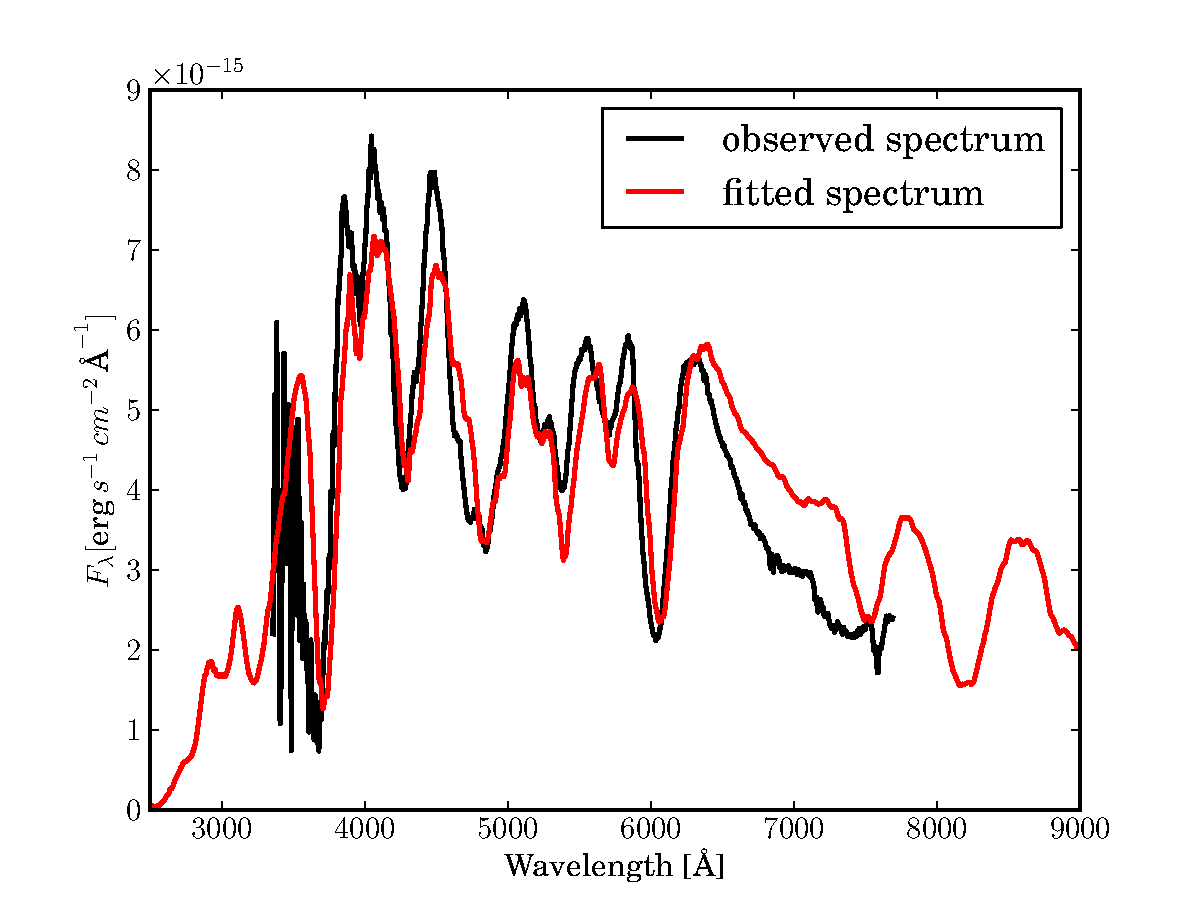
\includegraphics[width=\textwidth]{chapter_dalek/plots/bf2002bo-10.pdf} 
   \caption{example caption}
   \label{fig:sn2002bo-10_bf}
\end{figure}

The chosen fundamental parameters are $\loglbol=xx$, $\vph=xxx$. We have listed the non-zero abundances in Table \ref{tab:sn2002bo_perf_param}. 



The P-Cygni profiles of many features are easily visible. The Calcium line in the blue can be seen to be to blueshifted in relation to the model. This property is not unusual and is thought to come from high velocity component at the outer edge of the ejecta. The next major known discrepancy that can be seen is the excess of flux redwards of  $\approx 6200 \AA$.  This is a region that usually does not fit well as the underlying black body spectrum overestimates the flux in this region. When fitting manually often one tries to fit the depth the lines instead of the continuum.

There are three main parameters that have the most influence on the overall fit: Luminosity, photospheric velocity and abundance in iron group elements.

A large offset in \lum\ to the best fit paramater is easily visible as a large offset of the continuum (see Figure \ref{fig:sn2002bo_lum_offset}. Thus it is easy to constrain the parameter space in \lum\ initially. \lum\ also has influence on the temperature of the model through:
\[
L_{\rm bol} = 4\pi\sigma\, R^2\,T^4 = 4\pi\sigma\,\vph\,\texp.
\label{eq:lum_temp_relation}
\]

Velocity in astronomy is often measured using the doppler shift. In this case however it is hard to measure the photospheric velocity as lines are created at different depths and thus at different velocities. This smears out the line profiles which makes fitting velocities nearly impossible using this technique. 
The main impact of photospheric velocity is establishing the temperature given a luminosity. A model with a too high photospheric velocity will have expanded more than the real spectrum at that time and will be cooler. This results in a spectrum that is too luminous in the red and not luminous enough in the blue (see Figure \ref{fig:sn2002bo_vph_offset}). 
A secondary effect is that the ion population will be different to the actual supernova and the line spectrum differs.
\begin{figure}[htbp] %  figure placement: here, top, bottom, or page
   \centering
%   \includegraphics[width=2in]{replace} 
   \caption{example caption}
   \label{fig:sn2002bo_vph_offset}
\end{figure}
The initial abundances for each fit are determined by integrating the abundances above the photosphere in the W7 model \citep{1984ApJ...286..644N}.
The iron group element have a similar influence on the overall flux distribution as the photospheric velocity. 
As we assume no stable Cobalt and the input parameters for Nickel, Cobalt and Iron are $\Ni_0$ and $\Fe_0$ and calculate the abundances using radioactive decay. Ti and Cr have no easily identifiable single lines in the observed spectra, but provide line blanketing in the blue. We often lock their ratios and only use one abundance as an input parameter. 

These elements cause photons to be absorbed in the UV and be reemited in the red. A too high abundance will suppress the flux in the blue too much and will cause the spectrum to be over-luminous in the red (see Figure \ref{fig:sn2002_ige_offset}). Although physically different from the photospheric velocity, phenomenologically these are similar. 
The degeneracy is broken by identifiable Fe-Lines in the red part of the spectrum as well as the ionization balance determined by the temperature (influenced by photospheric velocity). 
This near degeneracy causes a very complex search space. 

There are six other abundances that are taken into account when fitting: Carbon, Oxygen, Magnesium, Silicon, Sulfur and Calcium. Among these Oxygen plays a special role. It does not have lines except the Oxygen triplet at 7778 \AA. In our fitting routine it acts as a buffer element and is assigned the remaining fraction that is left after all elements have been given abundances. 

The first element that is usually adjusted from its initial value is Calcium. The Calcium line is relatively easy to identify. Calcium also does not depend an awful lot on the right choice of temperature. One caveat however is that Calcium saturates at a certain point so if the observed line is close to that point one can only extract a lower limit for Calcium.

The next to be adjusted are Silicon and then Sulfur. Both of these elements are linked through nuclear synthesis and we don't expect there to be more Sulfur than Silicon. We also expect no less Sulfur than a third of Silicon. Silicon also provides an important measure for temperature through the ionization balance of doubly ionized Silicon to triple ionized Silicon (see Figure \ref{fig:sn2002bo_lineident}).


Magnesium has one strong feature near 4300 \AA, which constrains the Magnesium abundance. 

Doubly ionized Carbon has a line at $\approx 6300\,\AA$ which is often not present or very weak. 

Fitting the spectra involves first adjusting luminosity and then \ige s as well as photospheric velocity. This is followed by adjusting the other elemental abundances from the initial W7 values \citep{1984ApJ...286..644N}. After the elemental abundances are adjusted we readjust the luminosity, photospheric velocity and \ige again. This loop is continued until convergence is reached. 

One important factor to check is the value of the dilution factor $w$ at the photosphere. Theoretically we would expect this to be close to 0.5 if the fit is sensible. 

After having fit one spectrum we can continue to fit the other photpsheric spectra of the same supernova. We expect most parameters to increase or decrease monotonically (luminosity being the obvious exception). 

In summary, the fitting of a supernova is a complex procedure and requires a lot of practice. Our initial tests were using very simple methods like Newton-Raphson and other gradient methods. We quickly discovered the search space is too complex and evaluation time takes too long (each spectrum roughly one minute on a modern computer) to use these simple methods. 

 
\section{Genetic Algorithms}

Finding optimal solutions in complex search spaces is one of the main fields in numerical mathematics.  They have wide ranging applications in engineering, bio sciences and physical sciences. There have been several advances in the last decads to optimization. 
Among them is the  remarkable feat of ``solving'' the long-standing problem of the traveling salesman with simulated annealing \citep{Kirkpatrick13051983}.

\cite{Holland:1962:OLT:321127.321128}
Another major accomplishment was the development of evolutionary algorithms and subsequently genetic algorithms. The idea of an algorithm which imitates the principal of natural evolution was first introduced by ??? give story of rechenberg optimizing wind tunnel ??? Ingo Rechenberg \citep{Rechenberg1973}. These evolutionary algorithms have since become a sizeable subfield of numerical optimization. Genetic algorithms a subclass of evolutionary algorithms were then further developed by John Holland and David Goldberg \citep{citeulike:125978}.

When conquering the search space optimization algorithms have two (sometimes conflicting) goals: exploiting good leads while still exploring the search space sufficiently. Simple algorithms like Hillclimbing (randomly selecting a point in the neighbourhood and switch if it is ``better'' than the current one) will exploit good leads but will neglect to explore the search space. This often leads to be stuck at extrema. Whereas random searches are excellent at exploring the search space but will fail to quickly converge on an optimal solution. Genetic algorithms do strike the balance between exploration and exploiting the current best solution.
 """"
 maybe include:
 Dependent variables present special problems for optimization algorithms because varying one variable also changes the value of the other variable. For example, size and weight of the car are dependent. Increasing the size of the car will most likely increase the weight as well (unless some other factor, such as type of material, is also changed). Independent variables, like Fourier series coefficients, do not interact with each other. If 10 coefficients are not enough to represent a function, then more can be added without having to recalculate the original 10.
In the GA literature, variable interaction is called epistasis (a biological term for gene interaction). When there is little to no epistasis, minimum seeking algorithms perform best. GAs shine when the epistasis is medium to high, and pure random search algorithms are champions when epistasis is very high (Figure 2.5). cite haupt \& haupt (book on harddrive)
 """""""
Genetic algorithms are a heuristic search technique to find optimal solutions in n-dimensional search spaces. We will consider a function $f(\vec{x})$ with the multi-dimensional solution $\vec{y}$. In terms of genetic algorithms we call $\vec{x}$ genotypes and the solution vector $\vec{y}$ phenotype (similar to biology where the $\vec{x}$ describes the DNA sequence but the solution is can not be thought of as a vector). In addition we define a fitness function $g(\vec{y})=s$ where s is a scalar. It is our goal to choose the input parameters $\vec{x}$  to maximize $s$. 
Following the notation of \citep{Michalewicz:1994:GAD:184675} we introduce the population $P(t)$ with the individuals (sometimes referred to as genomes) $\{p_{1}^{t}, \dots, p_{n}^{t}\}$, where $t$ denotes the iteration. Each individual $(p_{i}^t)$ is a data structure consisting of a vector $\vec{x}_i$ and its corresponding fitness scalar $s_i$.  When we speak of evaluating $p_{i}^{t}$ we mean that we use $g(f(\vec{x}_i))=s_i$ to determine the fitness. A new population $P(t+1)$ is formed by choosing,  in the \textit{select step}, the more fit individuals. Some or all of the new population undergo transformations (recombine step). These transformations are called genetic operators. There are unary transformations, which create new individuals by small changes in single individuals called mutations. Higher order transformations called crossovers combine the traits of multiple individuals to form a next generation individual. 
After the new population has been created in the recombine step, it is evaluated and the \textit{select step} begins anew. 

This procedure is repeated until the best individual has reached a certain threshold fitness (see Algorithm \ref{alg:evol_program}). 



\begin{algorithm}
\label{alg:evol_program}
\caption{Structure of a genetic algorithm}
\begin{algorithmic}
\STATE $t \gets 0$\\
initialize $P(t)$\\
evaluate $P(t)$
\WHILE{(\textbf{not} termination condition)}
\STATE $t \gets t+1$\\
select $P(t)$ from $P(t-1)$\\
recombine $P(t)$\\
evaluate $P(t)$
\ENDWHILE
\end{algorithmic}
\end{algorithm}

To be solvable by a \ga the problem needs to meet the following requirements:
\begin{itemize}
\item a genetic representation of the search space (e.g. a vector)
\item a function that can calculate a fitness for a genetic representation
\item transformations that create a new population out of selected members of the old population
\item a method of creating an initial population
\end{itemize}


If these are fulfilled one can start constructing a \ga for the chosen problem. When constructing a new \ga for a problem there are multiple steps. First one needs to find a suitable genetic representation for each solution in the search space. 

\paragraph{Genetic Representation:}
There are two main ways to represent a genome: binary-encoding and value encoding (sometimes called gray encoding). Binary encoding was the form of encoding  used in early genetic algorithms. It offers significant advantages when trying to optimize very simple problems. 

In one-dimensional problems, for example, value encoding would only offer one gene, whereas binary encoding offers a number of genes depending on the requested precision of the value. 
There are however many problems with binary encoding. The so called \textit{hamming cliff} describes the problem that a simple bit-flip at one high encoding bit (occurring in some \ga\ operations) can dramatically change the encoded value \citet[e.g.][]{Chakraborty2003253}. This can improve covering of search space but also can hinder the code from converging quickly. When using binary encoding for many input variables the genomes can get incredibly large. \ga s have been shown to perform poorly for very large genomes. quicker convergence michalewicz page 82 chpter 5.5 

Value encoding often is a natural way to encode the parameters of a problem. In contrast to binary encoding the genetic operators are often much more problem specific. It seems that for the moment value encoding is the preferred method in many cases \citep[e.g.][]{Janikow1991Comparison,Wright91geneticalgorithms}.

Finally, an important encoding to mention (which does not apply to our example problem) is that of permutation encoding. In the famous case of the travelling salesman problem (henceforth \tsp) one tries to find the shortest route between n cities. In this case each city can only be visited once and the route must end in the starting city. There are many algorithms that can solve this problem. Brute force attempts scale with $O(n!)$ which make them unfeasible. A genetic algorithm can solve this problem by encoding the order (permutation encoding) in which the cities are visited in each genome. There are special genetic operators for permutation encoding. For the \tsp\ there are better algorithms like dynamic programming which can solve the problem with a complexity of $O(n^2 2^n)$ (see Figure \ref{fig:xkcd_tsp}).

\begin{figure}[htbp] %  figure placement: here, top, bottom, or page
   \centering
   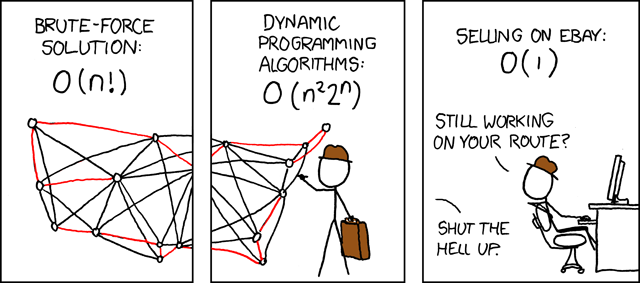
\includegraphics[width=0.7\textwidth]{chapter_dalek/plots/travelling_salesman_problem.png} 
   \caption{The death of the \tsp\ with the advent of online sales. (reproduced with kind permission by xkcd.com)}
   \label{fig:xkcd_tsp}
\end{figure}

In the case of a simple vectorized function or the \tsp\ once can now directly calculate the fitness value. In the case of our astrophysics example we need to first transform the genome (genotype) to a synthetic spectrum (phenotype) before being able to calculate the fitness.

\paragraph{Fitness Function}
Calculating the fitness of an individual is very dependent on the problem under consideration. In the case of our spectrum fitting problem we can simply calculate the root-mean-square for each individual. Finding a good fitness function in any optimization algorithm is one of the most complex tasks. It might not always be possible to find one fitness value that describes the problem but some problems might need many. This is generally referred to as multi-objective optimization and is an active field in \ga-research \citep{citeulike:1300532}. Fitness scaling applies a simple transformation to the fitness of all members of the population (e.g. a linear transform). Many selection processes are not able to accept negative and positive values for fitness so fitness scaling alleviates such a problem. In addition, it happens sometimes in early generation that a few individuals already have very high fitness. These "superindividuals" then dominate the selection process and subsequently reduce the genetic breadth  drastically. This can in later generations significantly hamper the progress of finding an optimal solution (such a problem was encountered in this work and is described in Section \ref{sec:geneticdalek}). 

In summary, fitness functions and scaling are a very crucial part of a successful algorithm. For a description of different scaling methods please refer to \citet{Kreinovich93geneticalgorithms} ??? select some introduction referebces from this paper???.

\paragraph{Initial Population}
The most basic method of selecting the initial population is to draw individuals uniformly and randomly from the entire search space. It depends then on the population size in relation to the search space size how well this search space is sampled. For a small population size and a large search space the \ga\ could very well find a local optimum rather than the global one. We have in our work chosen a population time which is roughly 15 times bigger than the number of genes. Choosing the initial population using prior knowledge will also improve the performance of the \ga. Rather than drawing uniformly random we would draw randomly from a probability distribution covering the search space. 

\paragraph{Selection process}
There are many different approaches for selecting individuals from the current population to create the next population. Before selecting individuals we can make coarse selection on the entire population. One selection that is often performed is that of \textit{elitism} in which a fraction of the fittest individuals is selected to advance to the next generation without being altered. On the other hand one can discard a fraction of the least fit individuals. These discarded members won't be used in the recombination step. The remaining population is called the mating population

After we have performed a coarse selection on the population we start with the recombination step. The first action in the recombination step is the selection of two or more individuals from the mating population and add them to a mating pool. In all our next examples we will assume a mating-pool with only two slots (similar to two parents in biological reproduction). Once the mating pool is filled a new individual is created by combining the genetic information of all members of the mating pool. 

There is a multitude of options for selecting members from the mating population and adding them to a mating pool \citep[for an overview see]{Goldberg91acomparative}. We will describe only a few of them. The most widely used of the selection algorithms is \textit{roulette wheel selection} (see Figure \ref{fig:roulettewheel}). \textit{Roulette wheel selection} is in the class of \textit{fitness proportional selection}. In addition to \textit{fitness proportional selection} there is \textit{rank selection}. In rank selection the fitness only influences the rank of the individuals (see Figure \ref{fig:rankselection}). The previous described fitness scaling and rank selection have similar effects. In \textit{tournament selection} we randomly select two individuals and compare those. The fitter of those two individuals is selected and added to the mating pool. 

There are multiple steps for creating a new population from the current mating population. First we select two individuals (or more) using our selection process (e.g. \textit{roulette wheel selection}) and place them in a mating pool. The reader should notice that the same individual can be in the mating pool twice! We create one or multiple new individuals (children) from this mating pool and place them in the new population. The current mating pool is disbanded and a new one is formed. These steps are repeated until the new population has the same number as the old population (minus the number of individuals that automatically advanced to the new population through \textit{elitism}). 
There are two main processes to create a new individual from a mating pool: crossover and mutation.
\begin{figure}[htbp] %  figure placement: here, top, bottom, or page
   \centering
   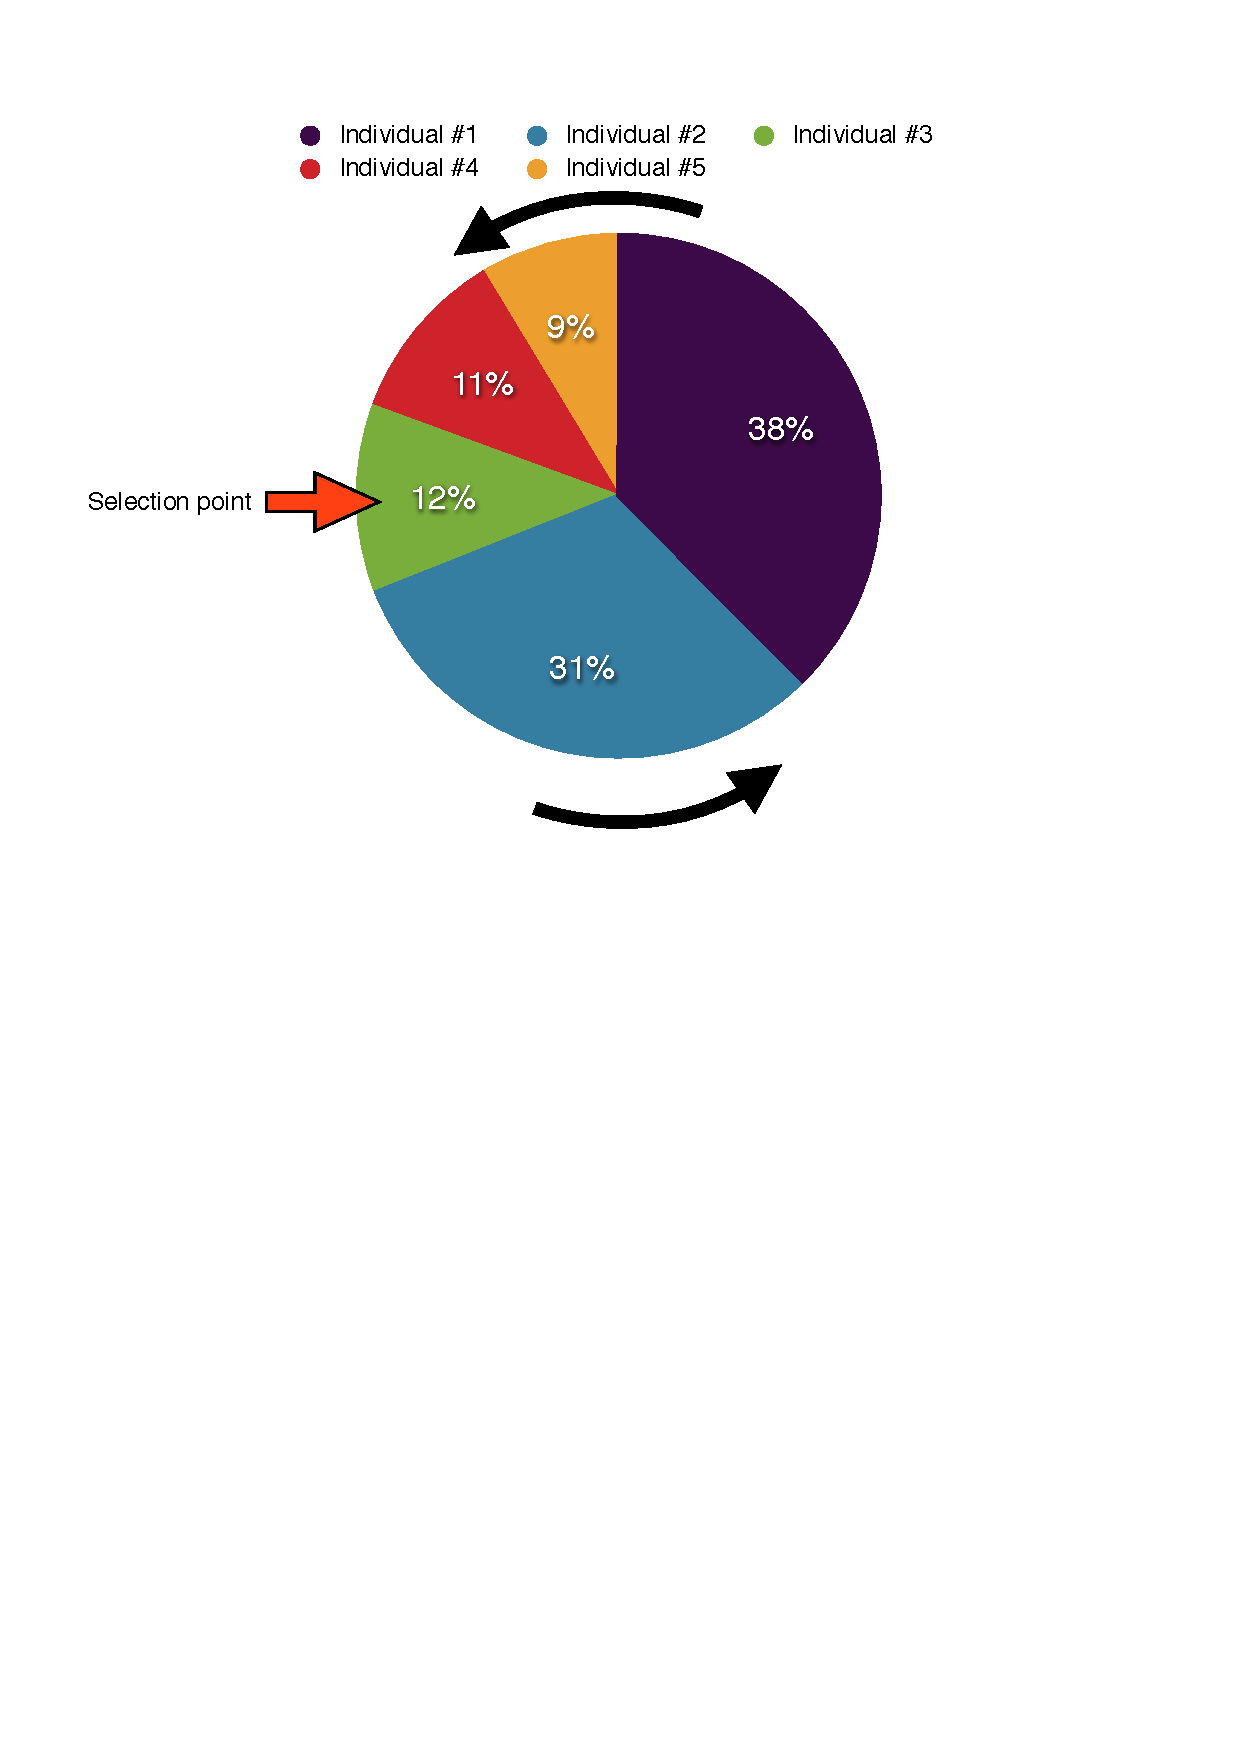
\includegraphics[width=0.7\textwidth]{chapter_dalek/plots/rws_cropped.pdf} 
   \caption{example caption}
   \label{fig:example}
\end{figure}

\paragraph{Crossover and mutation}
We assume a mating pool with two individuals. The simplest form of a crossover is the single-point crossover (see Figure \ref{fig:crossover}). A random integer $r \in [1,N-1]$, where N describes the number of genes per genome is selected. The new individual is created out of the first $r$ genes from the first parent and the last $N-r$ genes from the second parent. Now it is trivial to create a second child (using the same random number $r$) from the mating pool by just switching first and second parent. 
Two-point crossover is very similar to single-point crossover. Two random numbers are selected and the crossover occurs at these places (see Figure \ref{fig:crossover}). (N-1)-point crossover is also called uniform crossover. In that case each gene is selected randomly with equal chance from the parents.
Arithmetic crossovers use a function to calculate the new gene from each of the parent genes. For a value encoding this function could be the mean. For a binary encoding the function could be the \textit{and} operator. ???should I include example???
One can mix arithmetic and binary crossovers. For example we select the $r$ genes from the first parent and create the last $N-r$ genes by taking the mean of first and second parents genes. 
After the new child or children have been created through crossovers it is subjected to the mutation operator. There is a chance for each individual gene (often chosen to be less than 5\%) that it is altered. For bit encoding this altering is a simple inversions. There are many options for value encoding. For example one can add or multiply with a random number. 
Once this step is complete the children are added to the new population.

\subsection{A simple example}
We will illustrate the use of a \ga\ on a simple astrophysical problem. The task at hand is to fit an observed spectrum with a synthetic spectrum. The input parameters for this synthetic spectrum are\teff, \logg, \feh, $\alpha$-enhancement, \vrad and \vrot. The simplest genetic representation of this is simply a vector $\vec{x} = (\teff, \logg, \feh, \alpha, \vrad, \vrot)$. $\vec{x}$ is the \textit{genotype} of the individual. The resulting synthetic spectrum is called the \textit{phenotype}. 

For this relatively small number of genes a population size of 75 should suffice. The first step is drawing an initial population. We will draw uniformly randomly from the search space: $\teff \in [2000, 9000]$, $\logg \in [0, 5]$, $\feh \in [-5,1]$, $\alpha \in [0,0.4]$, $\vrad \in [-100, 100]$ and $\vrot \in [0,200]$. We compute the synthetic spectrum for each individual. The fitness of each individual is the inverse of the root-mean-square of the residuals between the observed and the synthetic spectrum. 
In the select step we will first advance 10 \% of the fittest individuals to the next population unaltered (\textit{elitism}). For the next population to be complete we need $75 - 8 = 67$ individuals which are created through mating. We select 2 individuals through \textit{roulette wheel selection} and place them in the mating pool. A single crossover point is randomly selected and the child is created. Before being placed in the new population the mutation operator is applied but has a very small chance to mutate any of the child's genes (in this case we choose 2\%).
This mating step (see Figure \ref{fig:example_mating}) is repeated 67 times. The new population now consists of the 8 fittest individuals of the old population and 67 new individuals created by mating. We will then start again to compute the synthetic spectrum and the resulting fitness for each individual of the new population. This loop is continued until one individual or a whole population has reached a preset convergence criterium.

\subsection{Convergence in Genetic Algorithms}
A key problem with all optimization algorithms is the premature convergence on a local optimum. The more complex the search space and the more interlinked the parameters are the more likely it is that traditional search routines will fail. \ga s are inherently better at bypassing local optima but are in no way immune to this problem. Premature convergence, as finding a local optimum is called in \ga-terms, is a well known problem 
A problem that is intrinsic to the \ga s is that for in traditional implementation they will never fully converge. The algorithm will get close to the optimum but due to continued mutation of the individuals the \ga\ will in most cases not reach it. To alleviate this problem some authors suggest switching to a different algorithm when close to the optimum solution, whereas others suggest changing the mutation rate over time \citep[see][and references therein]{citeulike:344183}.
A definite advantage of \ga s is their parallel nature. This makes it easy to explore large search spaces in the era of increasingly parallel computing. 

Although there are many advantages to using \ga s, one of the unsolved problems is determining a mathematical description for their convergence. The predominate schemata theory explains only a subset of the intrinsic complexity of \ga s.

\subsection{GA theory schemata theory}

The schemata-theory first described by \cite{holland1975} is one of the accepted theoretical interpretations of \ga s. There is some criticism and it is known that this theory only explains part of the complexity that are inherent to \ga s \citep[see ][ and references therein]{Whitley94agenetic}. 

\section{Genetic Algorithms to fit Type Ia Supernovae: The Dalek Code}
\label{sec:geneticdalek}
describe initial tries with newton raphson. 

Initial population. show vph graph. select from w7 integrate outwards. create children randomly; complex needs to work out and obey rules otherwise dead: describe process look at python code. ....

reference back to  parallelity and describe launching to multiple (non homogenious computers) simple fifo. 

fitness function describe chi**2 and then describe w-parameter and ir excess mention figure.

selection process rws; crossover uniform, mutation non-uniform different mutations for different parameters. child survival rate small at beginning.

describe principal evolution; show 2002bo different channels; population plot histtogram.
Fitting works sometime find good solution. discuss time and computer demand. discuss what has been tried

problems?

suggest that on the right way, now working with experts of genetic algorithms. describe differential evolution. 

ask james about machine learning techniques....

\section{Conclusion}



GA powerful tools, initially very good but require fine tuning for each problem.

A conventional, but not entirely accurate, interpretation of the NFL results is that "a general-purpose universal optimization strategy is theoretically impossible, and the only way one strategy can outperform another is if it is specialized to the specific problem under consideration"
http://ti.arc.nasa.gov/m/profile/dhw/papers/78.pdf

Continue on investigation with experts on GA. try some different approaches. Fast exploration of search space through grid and GA. 








\printglossaries
%\printglossary[type=gastro]
\bibliographystyle{astroads}
\phantomsection\addcontentsline{toc}{chapter}{Bibliography}
\bibliography{thesis}

\end{document}
